\documentclass[12pt]{beamer}

\usetheme[white,sections]{Wisconsin}
\usepackage{fancyvrb}
\usepackage{color}
\usepackage[normalem]{ulem}
\usepackage{xcolor}
\usepackage{anyfontsize}
\usepackage{wrapfig}
\usepackage{graphicx}
\usepackage{tikz}
\usetikzlibrary{shapes.arrows}
\tikzset{
    myarrow/.style={
        draw,
        fill=orange,
        single arrow,
        minimum height=2.5ex,
        single arrow head extend=0.5ex
    }
}
\tikzset{
    mydoublearrow/.style={
        draw,
        fill=orange,
        double arrow,
        minimum height=10.5ex,
        single arrow head extend=1ex
    }
}

\newcommand{\arrowup}{%
\tikz [baseline=-0.5ex]{\node [myarrow,rotate=90] {};}
}
\newcommand{\arrowdown}{%
\tikz [baseline=-1ex]{\node [myarrow,rotate=-90] {};}
}
\newcommand{\doublearrow}{%
\tikz [baseline=-1ex]{\node [mydoublearrow,rotate=0] {};}
}


\begin{document}
\newcommand*{\alphabet}{ABCDEFGHIJKLMNOPQRSTUVWXYZabcdefghijklmnopqrstuvwxyz}
\newlength{\highlightheight}
\newlength{\highlightdepth}
\newlength{\highlightmargin}
\setlength{\highlightmargin}{2pt}
\settoheight{\highlightheight}{\alphabet}
\settodepth{\highlightdepth}{\alphabet}
\addtolength{\highlightheight}{\highlightmargin}
\addtolength{\highlightdepth}{\highlightmargin}
\addtolength{\highlightheight}{\highlightdepth}
\setbeamertemplate{bibliography entry title}{}
\setbeamertemplate{bibliography entry location}{}
\setbeamertemplate{bibliography entry note}{}
\newcommand*{\Highlight}{\rlap{\textcolor{HighlightBackground}{\rule[-\highlightdepth]{\linewidth}{\highlightheight}}}}
\setbeamertemplate{bibliography item}[text]
\setbeamercolor{section in toc}{fg=white}
\setbeamercolor{bibliography entry author}{fg=black}
\setbeamercolor{bibliography item}{fg=black}
\setbeamercolor*{bibliography entry title}{fg=black}
%\setbeamerfont{section number projected}{size=\tiny}
\setbeamerfont{section number projected}{size=\fontsize{6}{6}\selectfont}
\setbeamercolor{section number projected}{bg=UWRed,fg=white}
\hypersetup{linkcolor=white,urlcolor=white}

\AtBeginSection{\frame{\sectionpage}}
\defbeamertemplate{section page}{mine}[1][]{%
  \begin{centering}
    {\usebeamerfont{section name}\usebeamercolor[fg]{section name}#1}
    \vskip1em\par
    \begin{beamercolorbox}[sep=12pt,center]{part title}
      \usebeamerfont{section title}\insertsection\par
    \end{beamercolorbox}
  \end{centering}
}
\setbeamertemplate{section page}[mine]

%%%%%%%%%%%%%%%%%%%%%%%%%%%%%%%%%%%%%%%%%%%%%%%%%%%%%%%%%%%%%%%%%%%%%%%%%%%%%%%%
\title{Quality Assurance within the PyNE Open Source Toolkit}   
\author{Elliott Biondo$^1$, Anthony Scopatz$^1$, Matthew Gidden$^1$, \\ 
        Rachel Slaybaugh$^2$, Cameron Bates$^2$, Paul P.H. Wilson$^1$}
\institute{$^1$University of Wisconsin - Madison \\ 
           $^2$University of California, Berkeley}
\date{Nov. 11, 2014}
\frame[plain]{\titlepage \addtocounter{framenumber}{-1}} 

%%%%%%%%%%%%%%%%%%%%%%%%%%%%%%%%%%%%%%%%%%%%%%%%%%%%%%%%%%%%%%%%%%%%%%%%%%%%%%%%
%%%%%%%%%%%%%%%%%%%%%%%%%%%%%%%%%%%%%%%%%%%%%%%%%%%%%%%%%%%%%%%%%%%%%%%%%%%%%%%%
%%%%%%%%%%%%%%%%%%%%%%%%%%%%%%%%%%%%%%%%%%%%%%%%%%%%%%%%%%%%%%%%%%%%%%%%%%%%%%%%
\section{Introduction}
%%%%%%%%%%%%%%%%%%%%%%%%%%%%%%%%%%%%%%%%%%%%%%%%%%%%%%%%%%%%%%%%%%%%%%%%%%%%%%%%
%%%%%%%%%%%%%%%%%%%%%%%%%%%%%%%%%%%%%%%%%%%%%%%%%%%%%%%%%%%%%%%%%%%%%%%%%%%%%%%%
%%%%%%%%%%%%%%%%%%%%%%%%%%%%%%%%%%%%%%%%%%%%%%%%%%%%%%%%%%%%%%%%%%%%%%%%%%%%%%%%
\begin{frame}[fragile]
\frametitle{The PyNE Toolkit}

\centerline{\bf Python for Nuclear Engineering:}
A trans-institutional, open source project for nuclear science and engineering analysis and similations.

\centerline{
\includegraphics[width=3cm]{figures/pyne_icon_small.png}}

\begin{itemize}
\item{A library of tools that can accomplish c}
\item{All code has a common Python interface}
\begin{itemize}
\item{A majority of code is written in C++ and wrapped with Python.}
\item{At one of GitHub.com's Top 25 ``trending'' C++ projects.}
\item{To date: 27 contributors, 21 with over 1000 lines of code/tests/documentation}
\end{itemize}
\end{itemize}


\end{frame}
%%%%%%%%%%%%%%%%%%%%%%%%%%%%%%%%%%%%%%%%%%%%%%%%%%%%%%%%%%%%%%%%%%%%%%%%%%%%%%%%
\begin{frame}[fragile]
\frametitle{The PyNE Toolkit}

\begin{columns}
\begin{column}{0.5\textwidth}
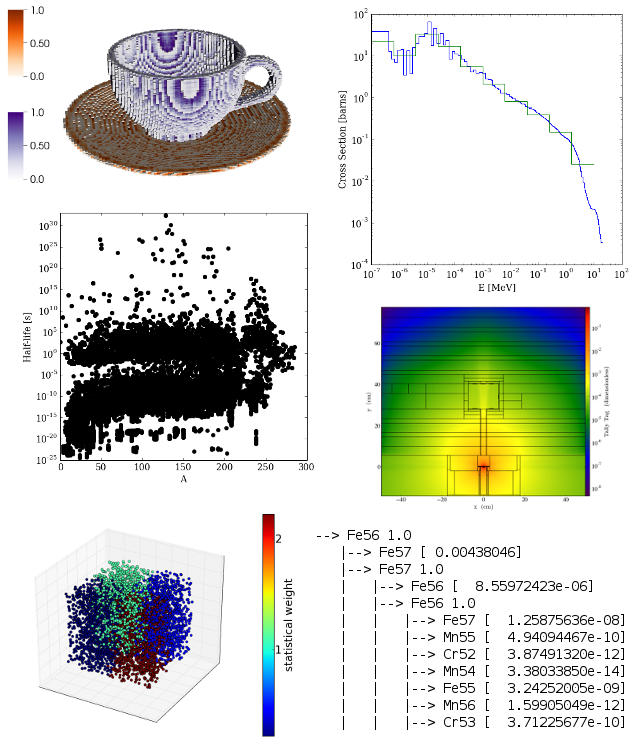
\includegraphics[width=\textwidth]{figures/pyne_splash.png}
\end{column}
\begin{column}{0.5\textwidth}
Core functionality:
\begin{itemize}
\item{Nuclide/reaction naming}
\item{Material handling}
\item{Mesh generation and operation}
\item{Cross section interface}
\item{Physics code support (MCNP5, Serpent, ALARA, ORIGEN 2.2)}
\item{Nuclear data (ACE, ENDF, ENSDF, CCCC, NJOY)}
\end{itemize}
\end{column}
\end{columns}

\end{frame}
%%%%%%%%%%%%%%%%%%%%%%%%%%%%%%%%%%%%%%%%%%%%%%%%%%%%%%%%%%%%%%%%%%%%%%%%%%%%%%%%
\begin{frame}
\frametitle{My work within PyNE}

\begin{columns}
\begin{column}{0.4\textwidth}
Mesh-based shutdown dose rate estimation for fusion energy systems \cite{Biondo2014}.
\begin{itemize}
\item{\texttt{mcnp}}
\item{\texttt{mesh}}
\item{\texttt{material} }
\item{\texttt{alara}}
\item{\texttt{dagmc}}
\item{\texttt{source sampling}}
\item{\texttt{variance reduction}}
\item{\texttt{r2s module}}
\end{itemize}
\end{column}
\begin{column}{0.6\textwidth}
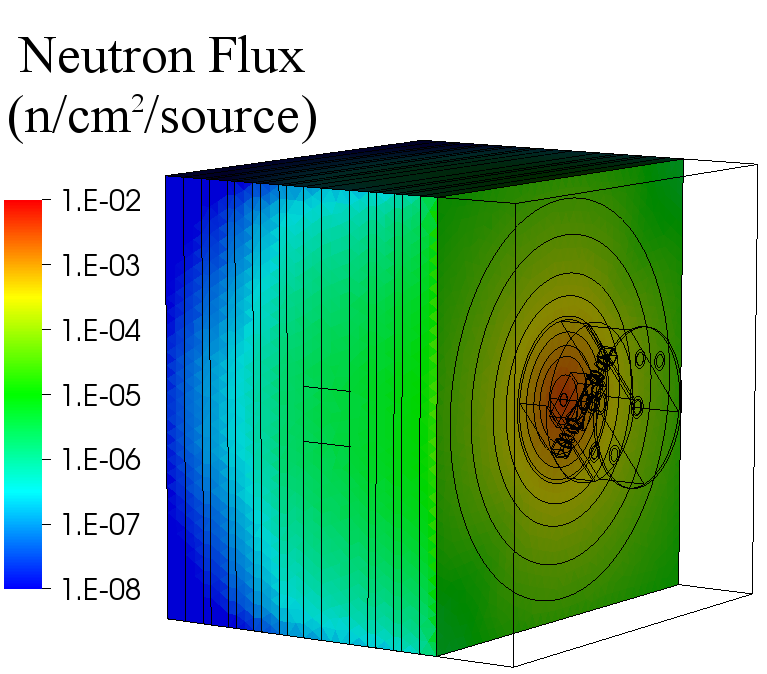
\includegraphics[width=3.8cm]{figures/n_flux.png}
\vspace{0.2cm}
{ \arrowdown} {\small Activation} \\
\centerline{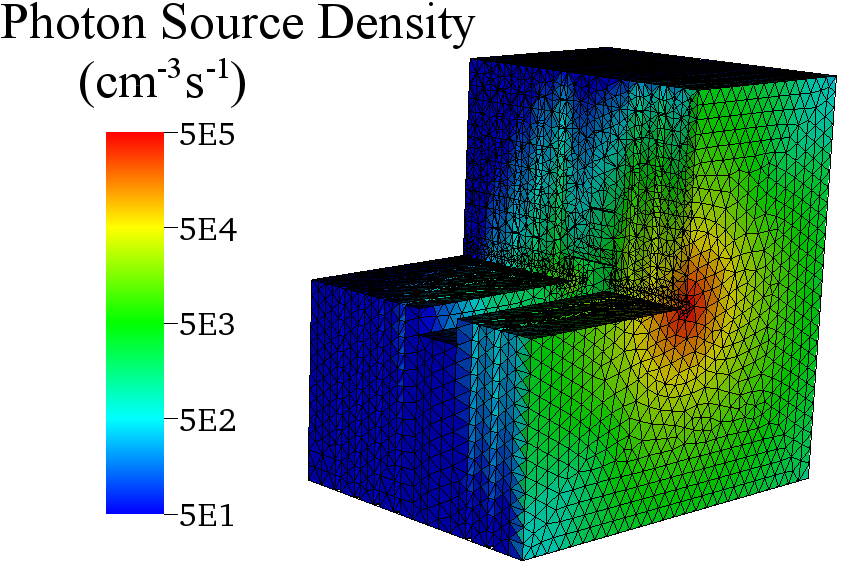
\includegraphics[width=4.2cm]{figures/phtn_src.png}}
\centerline{\hspace{0.5cm} \arrowdown {\small Photon Transport}} 
\vspace{0.2cm}
\framebox[1.1\width]{Shutdown Dose Rate}
\end{column}
\end{columns}
\end{frame}
%%%%%%%%%%%%%%%%%%%%%%%%%%%%%%%%%%%%%%%%%%%%%%%%%%%%%%%%%%%%%%%%%%%%%%%%%%%%%%%%
\begin{frame}[fragile]
\frametitle{Quality assurance}

\begin{itemize}
\item{PyNE developers have an interest in ensuring code is correct, robust,
well-documented, and easy to use.}
\item{Some activities within National Labs and industry require code that compliant with NRC regulatory standards.}
\begin{itemize}
\item{Increase potential user-base.}
\end{itemize}
\end{itemize}

\end{frame}
%%%%%%%%%%%%%%%%%%%%%%%%%%%%%%%%%%%%%%%%%%%%%%%%%%%%%%%%%%%%%%%%%%%%%%%%%%%%%%%%
\begin{frame}[fragile]
\frametitle{Quality assurance in nuclear engineering}

\begin{columns}[T]
\begin{column}{0.5\textwidth}

\includegraphics[width=\textwidth]{figures/nqa-1-2008.png}
\end{column}
\begin{column}{0.5\textwidth}
\begin{itemize}
\item{American Society of Mechical Engineers (ASME)
NQA-1-2008 \cite{nqa} standard and NQA-1a-2009 \cite{add} addendum}
\item{Endorsed by the NRC for design and construction of power plants and reprocessing facilities.}
\end{itemize}
\end{column}
\end{columns}


\end{frame}
%%%%%%%%%%%%%%%%%%%%%%%%%%%%%%%%%%%%%%%%%%%%%%%%%%%%%%%%%%%%%%%%%%%%%%%%%%%%%%%%
\begin{frame}[fragile]
\frametitle{The bottomline}

\begin{enumerate}
\item{What software development practices are enacted within PyNE for QA?}
\item{How do these practices map to the criteria set forth in NQA-1?}
\end{enumerate}


\end{frame}


%%%%%%%%%%%%%%%%%%%%%%%%%%%%%%%%%%%%%%%%%%%%%%%%%%%%%%%%%%%%%%%%%%%%%%%%%%%%%%%%
%%%%%%%%%%%%%%%%%%%%%%%%%%%%%%%%%%%%%%%%%%%%%%%%%%%%%%%%%%%%%%%%%%%%%%%%%%%%%%%%
%%%%%%%%%%%%%%%%%%%%%%%%%%%%%%%%%%%%%%%%%%%%%%%%%%%%%%%%%%%%%%%%%%%%%%%%%%%%%%%%
\section{NQA-1 Standards}
%%%%%%%%%%%%%%%%%%%%%%%%%%%%%%%%%%%%%%%%%%%%%%%%%%%%%%%%%%%%%%%%%%%%%%%%%%%%%%%%
%%%%%%%%%%%%%%%%%%%%%%%%%%%%%%%%%%%%%%%%%%%%%%%%%%%%%%%%%%%%%%%%%%%%%%%%%%%%%%%%
%%%%%%%%%%%%%%%%%%%%%%%%%%%%%%%%%%%%%%%%%%%%%%%%%%%%%%%%%%%%%%%%%%%%%%%%%%%%%%%%

\begin{frame}[fragile]
\frametitle{The Waterfall method \cite{waterfall}}
\centerline{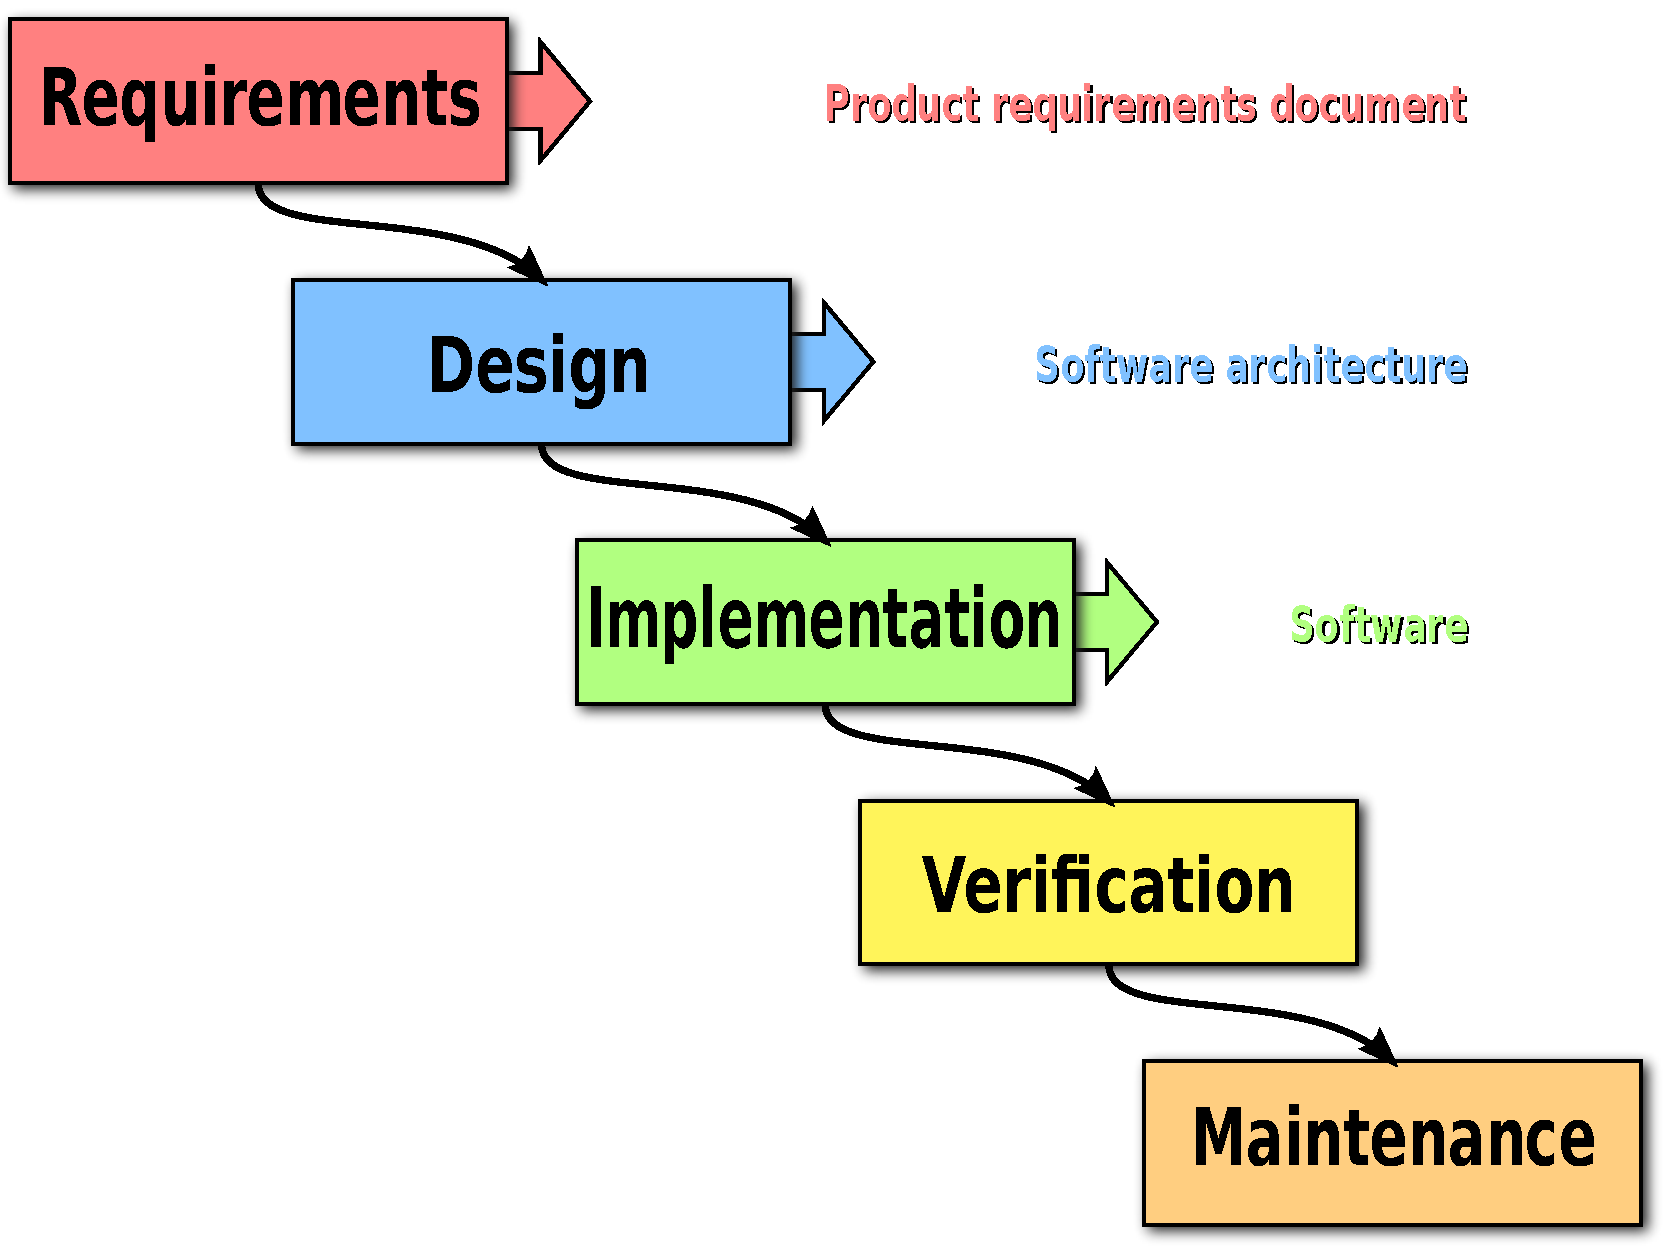
\includegraphics[width=0.8\textwidth]{figures/waterfall.pdf}}
Figure from \cite{waterfall_wiki}
\end{frame}


%%%%%%%%%%%%%%%%%%%%%%%%%%%%%%%%%%%%%%%%%%%%%%%%%%%%%%%%%%%%%%%%%%%%%%%%%%%%%%%%
\begin{frame}
\frametitle{The gist}

\begin{itemize}
\item{Use the Water Method}
\item{Document every step}
\end{itemize}

\end{frame}

%%%%%%%%%%%%%%%%%%%%%%%%%%%%%%%%%%%%%%%%%%%%%%%%%%%%%%%%%%%%%%%%%%%%%%%%%%%%%%%%
\begin{frame}
\frametitle{More concrete requirements}

Part I: “Requirements for Quality Assurance Programs for
Nuclear Facilities,

Pars. 801.1-801.5:
\begin{enumerate}
\item{Requirements - the scope of the capabilities implemented by the work.}
\item{Software design - the mathematical and computational methodologies employed to meet the requirements.}
\item{Implementation - writing code using the standards and conventions agreed upon by the organization.}
\item{Software design verification - independent confirmation that requirements are met.}
\item{Computer program testing - comparison of results produced by the work to expected or known results.}
\end{enumerate}

configuration identification - identify each version of the code and the difference between them
configuration change control - document changes to the baseline as well as justifiction/verification
configuration status control - accounted for prior to being incorporated into the baseline and changes that are “proposed and approved, but not implemented” are documented \cite{add}

\end{frame}

\begin{frame}
\frametitle{Part II}
Part II: “Quality Assurance Requirements for Facility Applications”

Otherwise Required Software

Reporting bug fixes, corrective action.
Security requirements
operations requirements
Documentations of standards, conventions, and work practices
System tools and system software


\end{frame}
%%%%%%%%%%%%%%%%%%%%%%%%%%%%%%%%%%%%%%%%%%%%%%%%%%%%%%%%%%%%%%%%%%%%%%%%%%%%%%%%



%%%%%%%%%%%%%%%%%%%%%%%%%%%%%%%%%%%%%%%%%%%%%%%%%%%%%%%%%%%%%%%%%%%%%%%%%%%%%%%%
\section{QA within PyNE}

\begin{frame}
\frametitle{QA within PyNE}
This is a developer's perspective -- users simily run their local unit tests.
\end{frame}


%%%%%%%%%%%%%%%%%%%%%%%%%%%%%%%%%%%%%%%%%%%%%%%%%%%%%%%%%%%%%%%%%%%%%%%%%%%%%%%%
\begin{frame}
\frametitle{Applicability of NQA-1}


Part II
Subpart 2.7 Section 302, “Otherwise Acquired Software.”
This section provides provisions for the use of “freeware”
that “has not been previously approved under a program
consistent with [the NQA-1 standard]”

Verify it yourself!

end-user application

Does physics occur? no physics in parsing and MCNP output file.


Part II Subpart 2.7 Section 302, “Otherwise Acquired Software.”

“freeware” that “has not been previously
approved under a program consistent with [the NQA-1 standard]”

Mapping our development process to NQA-1.

\end{frame}


%%%%%%%%%%%%%%%%%%%%%%%%%%%%%%%%%%%%%%%%%%%%%%%%%%%%%%%%%%%%%%%%%%%%%%%%%%%%%%%%
\begin{frame}[fragile]
\frametitle{Challenges}

\begin{itemize}
\item{PyNE developer are a diverse bunch}:
   \begin{itemize}
   \item{Undergraduates through tenured profesors.}
   \item{Varying levels of software development experience.}
   \item{Spare time vs. funded work -- effort.}
   \item{Research vs. production level.}
   \end{itemize}
\item{Agile Software Development \cite{larman2004agile}}
\end{itemize}

Software baseline
\end{frame}

%%%%%%%%%%%%%%%%%%%%%%%%%%%%%%%%%%%%%%%%%%%%%%%%%%%%%%%%%%%%%%%%%%%%%%%%%%%%%%%%
\begin{frame}
\frametitle{Documentation}
user manual
theory manual
\end{frame}

%%%%%%%%%%%%%%%%%%%%%%%%%%%%%%%%%%%%%%%%%%%%%%%%%%%%%%%%%%%%%%%%%%%%%%%%%%%%%%%%
\begin{frame}
\frametitle{Version Control}

\cite{git}

\end{frame}

%%%%%%%%%%%%%%%%%%%%%%%%%%%%%%%%%%%%%%%%%%%%%%%%%%%%%%%%%%%%%%%%%%%%%%%%%%%%%%%%
\begin{frame}
\frametitle{Pull Requests}

Developers create there own ``fork'', make changes there, and the requests that the changes get applied the baseline.

Formal review process by someone who did not write the code.

iterative process (pic)
I've had people I've never met before review my code.

~300 pull requests so far -- permitted saved 

\end{frame}

%%%%%%%%%%%%%%%%%%%%%%%%%%%%%%%%%%%%%%%%%%%%%%%%%%%%%%%%%%%%%%%%%%%%%%%%%%%%%%%%
\begin{frame}
\frametitle{Requirements for Pull Requests}
In order to be accepted:
\begin{itemize}
\item{Unit tests that cover any new features.}
\item{All preexisting}
\item{Inline documentation}
\item{Format compliant with the PyNE Style guide.}
\end{itemize}

\end{frame}



%%%%%%%%%%%%%%%%%%%%%%%%%%%%%%%%%%%%%%%%%%%%%%%%%%%%%%%%%%%%%%%%%%%%%%%%%%%%%%%%
\begin{frame}
\frametitle{Nightly testing Continuous Integration}

Nightly testing -- install PyNE's dependies, install PyNE, run the tests.
- PyNE mailing list is notified in the case of any failures.

Build and Test Lab (BatLab)

Ubuntu 12, Scientific Linux 6, Mac OSX 8, Ubuntu 10 with Python 3.

Continuous integration:

BatLab and GitHub connected with Polyphemus server


The automatic building and testing of code upon reciveing a pull request.

\cite{beck1998extreme}
\cite{batlab_2014}
\cite{polyphemus_2014}

\end{frame}


%%%%%%%%%%%%%%%%%%%%%%%%%%%%%%%%%%%%%%%%%%%%%%%%%%%%%%%%%%%%%%%%%%%%%%%%%%%%%%%%
\begin{frame}
\frametitle{The PyNE QA standard}

Currently applied to indiviual modules.

Everything heretofor has been the bare minimum to be accpeted into PyNE

The module has a theory manual entry that describes or cites all non-trivial mathematics and/or physics that occur within a module, and also lists the assumptions and limitations of the module.

The module is fully unit tested, with test coverage that spans the entire set of capabilities described in the theory manual. If the expected results of unit tests require non-trivial calculations, sample calculations should be provided in the theory manual. In other words, any numbers that appear in the unit tests must be reproducible.

The module has a user manual entry that describes how to use its functionality within the design basis.

If modules contain significant physics (e.g. transport, transmutation), the module must be benchmarked against experimental results, with appropriate uncertainty and sensitivity analysis. In addition, regression tests must be incorporated into the CI.

When removal of an import guard is proposed in a pull-request, both the requester and reviewer should be prepared to justify the decision to merge, in the event that the module falls under scrutiny.

\end{frame}


%%%%%%%%%%%%%%%%%%%%%%%%%%%%%%%%%%%%%%%%%%%%%%%%%%%%%%%%%%%%%%%%%%%%%%%%%%%%%%%%
\begin{frame}
\frametitle{Work to date}

Ratified Quality Assurance
One module fully complaint
Major topic at the PyNE 3 day Hack-a-thon at Berkeley this weekend.

\end{frame}


%%%%%%%%%%%%%%%%%%%%%%%%%%%%%%%%%%%%%%%%%%%%%%%%%%%%%%%%%%%%%%%%%%%%%%%%%%%%%%%%
\begin{frame}[fragile]
\frametitle{Acknowledgements}


\includegraphics[height=2cm]{figures/NRClogo.png} \\

\end{frame}

%%%%%%%%%%%%%%%%%%

%%%%%%%%%%%%%%%%%%%%%%%%%%%%%%%%%%%%%%%%%%%%%%%%%%%%%%%%%%%%%%%%%%%%%%%%%%%%%%%%
%%%%%%%%%%%%%%%%%%%%%%%%%%%%%%%%%%%%%%%%%%%%%%%%%%%%%%%%%%%%%%%%%%%%%%%%%%%%%%%%
%%%%%%%%%%%%%%%%%%%%%%%%%%%%%%%%%%%%%%%%%%%%%%%%%%%%%%%%%%%%%%%%%%%%%%%%%%%%%%%%
\section*{Questions?}
%%%%%%%%%%%%%%%%%%%%%%%%%%%%%%%%%%%%%%%%%%%%%%%%%%%%%%%%%%%%%%%%%%%%%%%%%%%%%%%%
%%%%%%%%%%%%%%%%%%%%%%%%%%%%%%%%%%%%%%%%%%%%%%%%%%%%%%%%%%%%%%%%%%%%%%%%%%%%%%%%
%%%%%%%%%%%%%%%%%%%%%%%%%%%%%%%%%%%%%%%%%%%%%%%%%%%%%%%%%%%%%%%%%%%%%%%%%%%%%%%%

%\begin{frame}[allowframebreaks]
\begin{frame}[plain]
        \tiny
        \frametitle{References}
        \bibliographystyle{ans}
        \color{black}
        \bibliography{refs}
\end{frame}

%%%%%%%%%%%%%%%%%%%%%%%%%%%%%%%%%%%%%%%%%%%%%%%%%%%%%%%%%%%%%%%%%%%%%%%%%%%%%%%%
%%%%%%%%%%%%%%%%%%%%%%%%%%%%%%%%%%%%%%%%%%%%%%%%%%%%%%%%%%%%%%%%%%%%%%%%%%%%%%%%
%%%%%%%%%%%%%%%%%%%%%%%%%%%%%%%%%%%%%%%%%%%%%%%%%%%%%%%%%%%%%%%%%%%%%%%%%%%%%%%%
\end{document}
%%%%%%%%%%%%%%%%%%%%%%%%%%%%%%%%%%%%%%%%%%%%%%%%%%%%%%%%%%%%%%%%%%%%%%%%%%%%%%%%
%%%%%%%%%%%%%%%%%%%%%%%%%%%%%%%%%%%%%%%%%%%%%%%%%%%%%%%%%%%%%%%%%%%%%%%%%%%%%%%%
